

\chapter{System Overview}


\section{System Architecture}
\label{sec:architecture}
Our system consumes as an input\footnote{In practice, the aggregated input events stream is composed of multiple event streams (partitions) from a set of moving objects.} an aggregated stream of events coming from a large number of moving objects, which is continuously collected and fed into the system. It allows users to register a pattern $\mathcal{P}$ to be monitored over each event stream of a moving object. The output stream consists of original input events and predictions of full matches of $\mathcal{P}$, displayed to the end users. Figure ~\ref{fig:architecture} presents the overview of our system architecture and its main components.      


\begin{figure}[h]
	
	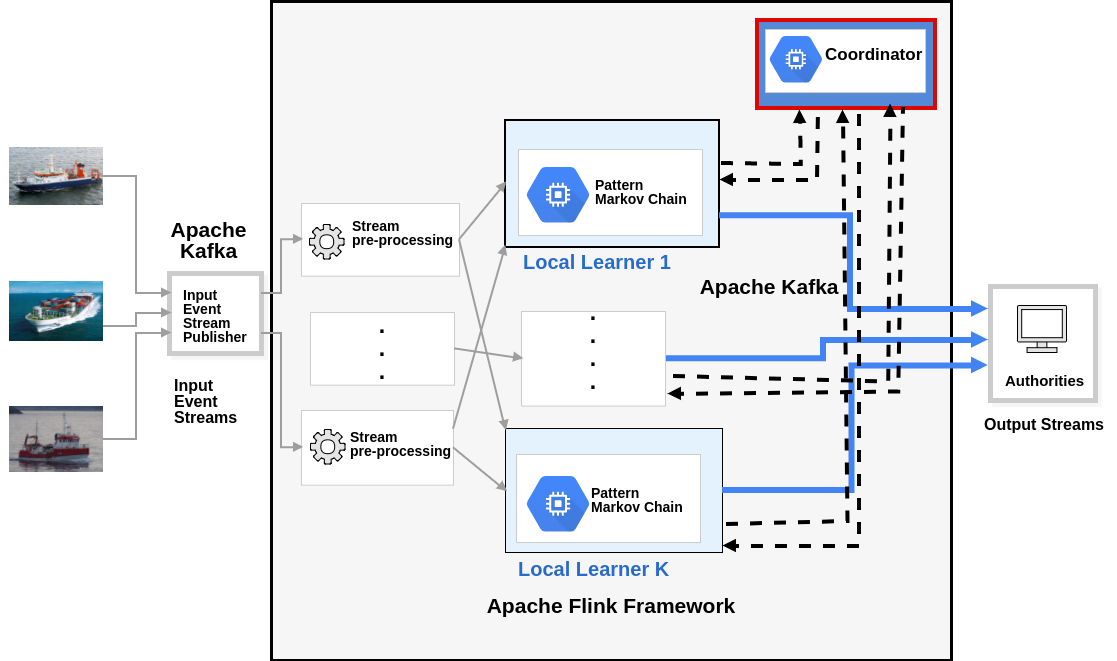
\includegraphics[width=\linewidth]{chapters/figures/distributed_architecture_f.png}
	
	\caption{System architecture overview.}
	\label{fig:architecture}
\end{figure}

The system is composed of three processing units:   \begin{enumerate}[]
	\item pre-processing operators that receive the input event stream and perform filtering and ordering operations, before partitioning the input event stream to multiple event streams based on the associated moving object 
	\item predictor nodes (learners), which are responsible for maintaining a prediction model for the input event streams. Each prediction node is configured to handle an event stream from the same moving object, in order to provide online predictions for a predefined pattern $\mathcal{P}$  
	\item a coordinator node that communicates through Kafka stream channels with the predictors to realize the distributed online learning protocol. It builds a global prediction model, based on the received local models, and then shares it among the predictors.
\end{enumerate}

\par Our distributed system consists of multiple pre-processing operators, prediction nodes, and a central coordinator node. All units run concurrently and are arranged as a  data processing pipeline, depicted in Figure ~\ref{fig:architecture}. We leverage Apache Kafka as a messaging platform to ingest the input event streams and to publish the resulting streams. Also, it is used as the communication channel between the predictor nodes and the coordinator. Apache Flink is employed to execute the system's distributed processing units over the input event streams: the pre-processing operators,  the prediction units, and the coordinator node. Our system architecture can be modeled as a logical network of processing nodes, organized in the form of a DAG, inspired by the Flink runtime dataflow programs \cite{carbone2015apache}. 

\section{Implementation Details}
\label{sec:impl}
In this section, we describe in detail the implementation of our system. It has been implemented on top of Apache Flink and Apache Kafka frameworks. Each of the three sub-modules, described in Section ~\ref{sec:architecture}, have been implemented as Flink operations over the input events stream. 

\textbf{Pre-processing and Prediction Operators.} Listing ~\ref{algonline:flink1} shows how the main workflow of the system is implemented as Flink data flow program.

The system ingests the input events stream from a Kafka cluster that is mapped to a \textit{DataStream} of events, which is then processed by an \textit{EventTuplesMapper} to create tuples of \textit{(id, event)}, where the \textit{id} is associated to the identifier of the moving object. To handle events  coming in out of order in a certain margin, the stream of event tuples  is processed by a \textit{TimestampAssigner}, it assigns the timestamps for the input events based on the extracted creation time. Afterwards,  an ordered stream of event tuples is generated using a process function \textit{EventSorter}.

	\begin{lstlisting}[caption={Flink pipeline for local predictors workflow},label={algonline:flink1},frame=single]
	DataStream<Event> eventsStream = env.addSource(kafkaConsumer);	
	// Create event tuples (id,event) and assign time stamp 
	DataStream<Tuple2<String,Event>> eventTuplesStream =
	inputEventsStream.map(new EventTuplesMapper())
	.assignTimestampsAndWatermarks(new EventTimeAssigner());	
	// Create the ordered keyed stream 
	 keyedEventsStream = eventsStream.keyBy(0).process(new EventSorter()).keyBy(0);	
	//Initialize the predictor node 
	LocalPredictorNode predictorNode =new LocalPredictorNode<Event>(P);
	// Process the  keyedEventsStream by the predictor 
	DataStream<Event> processedEventsStream =
	keyedEventsStream.map(predictorNode);
	\end{lstlisting}
	
 The ordered stream is then transformed to a \textit{keyedEventsStream} by partitioning it, based on the ids values, using a \textit{keyBy} operation. A local \textit{predictor} node in a distributed environment is represented by a \textit{map} function over the \textit{keyedEventsStream}. Each parallel instance of the map operator (predictor) always processes all events of the same moving object (i.e., equivalent id), and maintains a bounded prediction model (i.e., \pmcmr\  predictor) using the Flink's Keyed State  \footnote{{Keyed State in Flink: \url https://ci.apache.org/projects/flink/flink-docs-release-1.3/dev/stream/state.html\#kayed-state}}.  The output streams of the moving objects from the parallel instances of the predictor map functions are sent to a new Kafka stream (i.e., same topic name).  They then can be processed by other components like visualization or users notifier.


\par Moreover, the implementation of  the \textit{predictor} map function includes the communication  with \textit{coordinator} using Kafka streams. At the beginning of the execution, it sends a registration request to the coordinator. Also at the run-time,  it sends  its local prediction model as synchronization request,  or as a response for a resolution request from the coordinator. These communication messages are published into different Kafka topics as depicted in Table ~\ref{tab:messagesToTopics}. 

\begin{table}[h]
	\caption{Messages to Kafka topics mapping.}
	\label{tab:messagesToTopics}
	\begin{tabular}{p{3cm}l}
		\toprule
		Message &Kafka Topic\\
		\midrule
		\parbox[t]{4cm}{\textit{RegisterNode}, \\ \textit{RequestSync}, and \\\textit{ResolutionAnswer} } &LocalToCoordinatorTopicId\\ \\
		
			  \parbox[t]{4cm}{\textit{CoordinatorSync} and \\ \textit{RequestResolution}} &CoordinatorToLocalTopicId\\
		\bottomrule
	\end{tabular}
\end{table}


\textbf{Coordinator.} Listing ~\ref{algonline:flink2} presents the workflow of the coordinator node that manages the distributed online learning protocol operations, which is implemented as Flink program. The coordinator receives messages from the local predictors through a Kafka Stream of a topic named \textit{"LocalToCoordinatorTopicId"}. It is implemented as a single \textit{map} function over the messages stream, by setting the \textit{parallelism} level of the Flink program to \textit{"1"}. Increasing the parallelism will scale up the number of parallel coordinator instances, for example, in order to handle different groupings of the input event streams. The map operator of the coordinator  handles three message types from the predictors: \begin{enumerate}[]
	\item \textbf{RegisterNode} that contains  a registration request for a new predictor node,
	\item \textbf{RequestSync} to receive a local model after violation,
	\item \textbf{ResolutionAnswer} to receive a resolution response from a local predictor node.  
\end{enumerate}  
 In addition, it sends \textbf{CoordinatorSync} messages for all predictors after creating a new global prediction model, or \textbf{RequestResolution} to a ask the local predictors for their prediction models.
 

\begin{lstlisting}[caption={The coordinator Flink program.},label={algonline:flink2},frame=single]	
    streamExecutionEnvironment.setParallelism(1);
	// Read messages from local predictors
	DataStream<TopicMessage> messagesStream = readKafkaStream(env, "LocalToCoordinatorTopicId");	
	// Initialize the coordinator node
	CompunctionEfficientCoordinator coordinatorNode = new CompunctionEfficientCoordinator(configs);
	// Ingest the messages stream by the coordinator	
	DataStream<CoordinatorMessage> coordinatorMessagesStream = messageStream.map(coordinatorNode);	
	// Send the messages from the coordinator to the local predictors
	writeKafkaStream(coordinatorMessagesStream, CoordinatorToLocalTopicId);
\end{lstlisting}
       